\section{伪随机生成器}

回顾一下一次性密码本。在这里,密钥、消息和密文都是 $L$ 比特字符串。然而,我们实际希望使用一个更短的密钥。因此,我们的想法是使用一个短的、$\ell$ 比特的``种子" $s$ 作为加密密钥,其中 $\ell$ 的长度比 $L$ 短得多,然后将这个种子``拉伸"成一个较长的、$L$比特的字符串,用来掩盖消息(和解除对密文的掩盖)。拉伸种子 $s$ 需要使用某个有效的确定性算法 $G$,该算法能够将任意 $\ell$ 比特字符串映射成 $L$ 比特字符串。因此,这种修改后的一次性密码本的密钥空间为 $\{0,1\}^\ell$,而消息空间与密文空间仍为 $\{0,1\}^L$。对于$s\in\{0,1\}^\ell$ 和 $m,c\in\{0,1\}^L$,加密和解密的定义如下:
$$
E(s,m):=G(s)\oplus m,\quad
D(s,c):=G(s)\oplus c
$$
这种修改后的一次性密码本被称作一种\textbf{流密码(stream cipher)},而函数 $G$ 被称为\textbf{伪随机生成器 (pseudo-random generator)}。

如果 $\ell<L$,那么根据香农定理,这种流密码肯定不能实现完美安全性。但是如果 $G$ 满足适当的安全属性,这种密码也能达到语义安全。假设 $s$ 是一个随机的 $\ell$ 比特字符串,$r$ 是一个随机的 $L$ 比特字符串。直观地说,如果一个对手无法有效区分出 $G(s)$ 与 $r$ 的区别,他应该就不能分辨出流密码与传统的一次性密码本之间的区别;此外,既然后者的密码是语义安全的,那么前者自然也是语义安全的。为了使上述推理更加严谨,我们需要将对手不能``有效区分 $G(s)$ 与 $r$之间的差异"这一概念形式化。

一种用于区分伪随机字符串 $G(s)$ 和真随机字符串 $r$ 的算法称为\textbf{统计检验(statistical test)}。它把一个字符串作为输入,并输出 $0$ 或 $1$。如果它在伪随机输入上输出 $1$ 的概率与在真正随机输入上输出 $1$ 的概率有显著差异,那么这样的检验就被称作是\textbf{有效的}。即便是相对较小的概率差异,比如说 $1\%$,也被认为是显著的;事实上,即使只有 $1\%$ 的差异,如果我们能够获得几百个独立的样本,这些样本要么都是伪随机的,要么就都是真随机的,那么我们就能够很有把握地推断出我们所看到的到底是伪随机字符串还是真随机字符串。但是,一个非零但是可忽略不计的概率差异,比如$2^{-100}$,就是没有帮助的。

如何去设计一个有效的统计检验呢?一个基本的方法是:给定一个 $L$ 比特字符串,计算一些统计量,然后看看如果我们认为这个字符串是真随机的话,这个统计量与我们的预期是否存在较大的差异。

例如,一个非常简单的、很容易计算的统计量是字符串中出现的 $1$ 的次数 $k$。对于一个真随机的字符串,我们认为 $k\approx{L}/{2}$。如果PRG $G$ 对$1$ 或者 $0$有一些偏向性,我们就可以通过一个统计检验有效地检测到这一点,比如说,如果 $|k-0.5L|<0.01L$,则输出 $1$,否则就输出 $0$。

前面例子中的检验还可以加强,我们不仅仅可以考虑单个比特,还能够考虑成对的比特。我们可以将 $L$ 比特字符串分解成 $\approx{L}/{2}$ 个比特对,并统计 $00$ 对出现的次数 $k_{00}$,$01$ 对出现的次数 $k_{01}$,$10$ 对出现的次数 $k_{10}$,以及 $11$ 对出现的次数 $k_{11}$。对于一个真随机字符串,我们会预期上面的这四个统计量都 $\approx{L}/{8}$。因此,一个自然的统计检验是检验这些统计量与 ${L}/{8}$ 的偏差是否小于某个指定界限。或者,我们也可以将这些偏差的平方相加,并检验这个和是否小于某个指定的界限,这就是统计学中经典的 $\chi$ 方检验。

我们还可以检查其他的许多简单的统计量。然而,像这样的简单检验并没有倾向于利用算法 $G$ 的更深层次的数学特性,而恶意对手在设计专门针对 $G$ 的攻击时可能会利用这些特性。比如说,对于有一些PRG,上面的简单检验对其完全无效,但当给定足够多的输出比特时,其模式是完全可以预测的;也就是说,给定 $G(s)$ 的一个足够长的前缀,对手就可以计算出 $G(s)$ 的所有剩余比特,甚至能够计算出种子 $s$ 本身。

我们对 PRG 的安全性的定义正式给出了不应该有有效的(和可有效计算的)统计检验的概念。

\subsection{伪随机生成器的定义}

\textbf{伪随机生成器(pseudo-random generator)},简称\textbf{PRG},是一个有效确定性算法 $G$,以一个种子 $s$ 作为输入,计算并输出一个值 $r$。种子 $s$ 来自一个有限的种子空间 $\mathcal{S}$,而输出 $r$ 属于一个有限的输出空间 $\mathcal{R}$。通常情况下,$\mathcal{S}$ 和 $\mathcal{R}$ 是一些定长比特串的集合(例如,在上面的讨论中,我们有$\mathcal{S}=\{0,1\}^\ell$和$\mathcal{R}=\{0,1\}^L$)。我们称 $G$ 是一个定义在 $(\mathcal{S},\mathcal{R})$ 上的 PRG。

我们对 PRG 的安全定义抓住了这样一个直观的概念:如果 $s$ 是从 $\mathcal{S}$ 中随机选择的,而 $r$ 是从 $\mathcal{R}$ 中随机选择的,那么任何有效对手都无法有效地分辨 $G(s)$ 和 $r$ 之间的区别:两者是\textbf{计算上不可区分(computationally indistinguishable)}的。该定义被表述为一个攻击游戏。

\begin{game}[伪随机生成器]\label{game:3-1}
对于一个定义在 $(\mathcal{S},\mathcal{R})$ 上的给定 PRG $G$ 和一个给定的对手 $\mathcal{A}$,我们定义两个实验:实验$0$和实验$1$。对于 $b=0,1$,我们定义:

\noindent\textbf{实验 $b$:}
\begin{itemize}
	\item 挑战者按如下方式计算 $r\in\mathcal{R}$:
	\begin{itemize}
		\item 如果 $b=0$:$s\overset{\rm R}\leftarrow\mathcal{S}$,$r\leftarrow G(s)$;
		\item 如果 $b=1$:$r\overset{\rm R}\leftarrow\mathcal{R}$。
	\end{itemize}
	然后将 $r$ 发送给对手。
	\item 给定$r$,对手计算并输出一个比特 $\hat{b}\in\{0,1\}$。
\end{itemize}

对于 $b=0,1$,定义 $W_b$ 是 $\mathcal{A}$ 在实验 $b$ 中输出 $1$ 的事件。我们定义 $\mathcal{A}$ 对于 $G$ 的\textbf{优势}为:
$$
{\rm PRG\mathsf{adv}}[\mathcal{A},G]:=|{\rm Pr}[W_0]-{\rm Pr}[W_1]|
$$
\end{game}

该攻击游戏如图 \ref{fig:3-1} 所示。

\begin{figure}
  \centering
  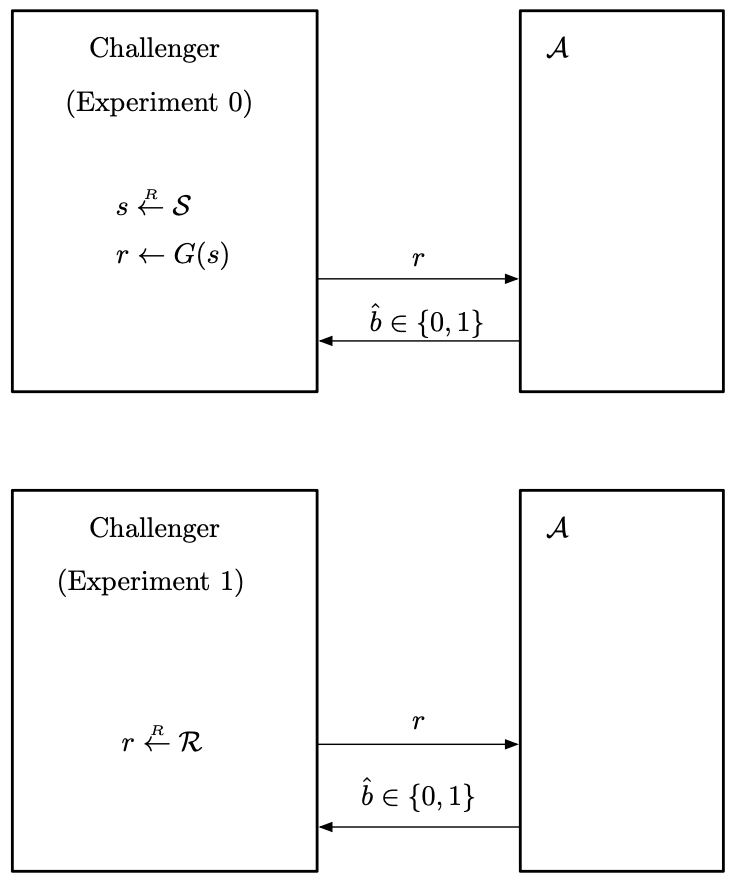
\includegraphics[width=0.5\linewidth]{figures/chapter3/fig1.png}
  \caption{攻击游戏 \ref{game:3-1} 的实验$0$和实验$1$}
  \label{fig:3-1}
\end{figure}

\begin{definition}[安全的 PRG]\label{def:3-1}
如果对于所有有效对手 $\mathcal{A}$,${\rm PRG\mathsf{adv}}[\mathcal{A},G]$ 的值都可忽略不计,我们就称 PRG $G$ 是\textbf{安全的}。

\end{definition}

正如 \ref{subsec:2-2-5} 小节所讨论的,攻击游戏 \ref{game:3-1} 可以被重构为一个``比特猜测"游戏,挑战者不再进行两个独立的实验,而是随机选择 $b\in\{0,1\}$,然后针对对手 $\mathcal{A}$ 运行实验 $b$。在这个游戏中,我们记$\mathcal{A}$ 的\emph{比特猜测优势}${\rm PRG\mathsf{adv}}^*[\mathcal{A},G]$ 为 $|\Pr[\hat b=b]-{1}/{2}|$。\ref{subsec:2-2-5} 小节中的一般结论(即式 \ref{eq:2-11})在此也适用:
\begin{equation}
{\rm PRG\mathsf{adv}}[\mathcal{A},G]=2\cdot{\rm PRG\mathsf{adv}}^*[\mathcal{A},G]
\end{equation}

我们还注意到,只有当种子空间的势(cardinality)是超多项式的时候,PRG 才是安全的(见练习3.5)。

\subsection{数学细节}

如 \ref{sec:2-3} 节一样,我们在这里给出更多与 PRG 有关的数学细节。就像 \ref{sec:2-3} 节一样,读者在初读这一小节时可以安全地跳过,在理解上也不会有什么损失。

首先,我们使用定义 \ref{def:2-9} 中介绍的术语来精确定义 PRG。

\begin{definition}[伪随机生成器]
一个伪随机生成器包括一个算法 $G$ 和两个具有系统参数化 $P$ 的空间族:
$$
\mathbf{S}=\{\mathcal{S}_{\lambda,\Lambda}\}_{\lambda,\Lambda},\quad
\mathbf{R}=\{\mathcal{R}_{\lambda,\Lambda}\}_{\lambda,\Lambda}
$$
满足:
\begin{enumerate}
	\item $\mathbf{S}$ 和 $\mathbf{R}$ 是可有效识别和可有效采样的。
	\item 算法 $G$ 是一个有效确定性算法,对于输入 $\lambda,\Lambda,s$,其中 $\lambda\in\mathbb{Z}_{\geq1}$,$\Lambda\in{\rm Supp}(P(\lambda))$,$s\in\mathcal{S}_{\lambda,\Lambda}$,它输出 $\mathcal{R}_{\lambda,\Lambda}$ 中的一个元素。
\end{enumerate}
\end{definition}

接下来,我们需要对定义 \ref{def:3-1} 进行正确的解释。首先,在攻击游戏 \ref{game:3-1} 中,需要理解的是,对于安全参数 $\lambda$ 的每个可能取值,我们都能得到一个不同的概率空间,该空间由挑战者的随机选择和对手的随机选择共同决定。其次,挑战者会产生一个系统参数 $\Lambda$,并在游戏一开始时就将其发送给对手。第三,优势 ${\rm PRG\mathsf{adv}}[\mathcal{A},G]$ 是安全参数 $\lambda$ 的一个函数,安全性则意味着该函数是一个可忽略不计函数。